\documentclass[12pt]{article}
\usepackage{epsfig}
\usepackage{url}
\usepackage{fancyhdr}
\usepackage{listings}
\usepackage{color}
\definecolor{commentsRGB}{rgb}{0.13,0.55,0.13}
\definecolor{stringsRGB}{rgb}{0.63,0.125,0.94}


\lstloadlanguages{C++}

\lstset{
keywordstyle = \color{blue},
identifierstyle =, 
commentstyle = \color{commentsRGB}, 
stringstyle = \ttfamily \color{stringsRGB},
language = {C++},
extendedchars = true, 
breaklines = true,
breakautoindent = true,
breakindent = 30pt,
}


\date{}
\author{}
\title{MyServer development model}

\begin{document}
\maketitle
\thispagestyle{empty}

\newpage

\begin{figure}[H]
  \begin{center}
    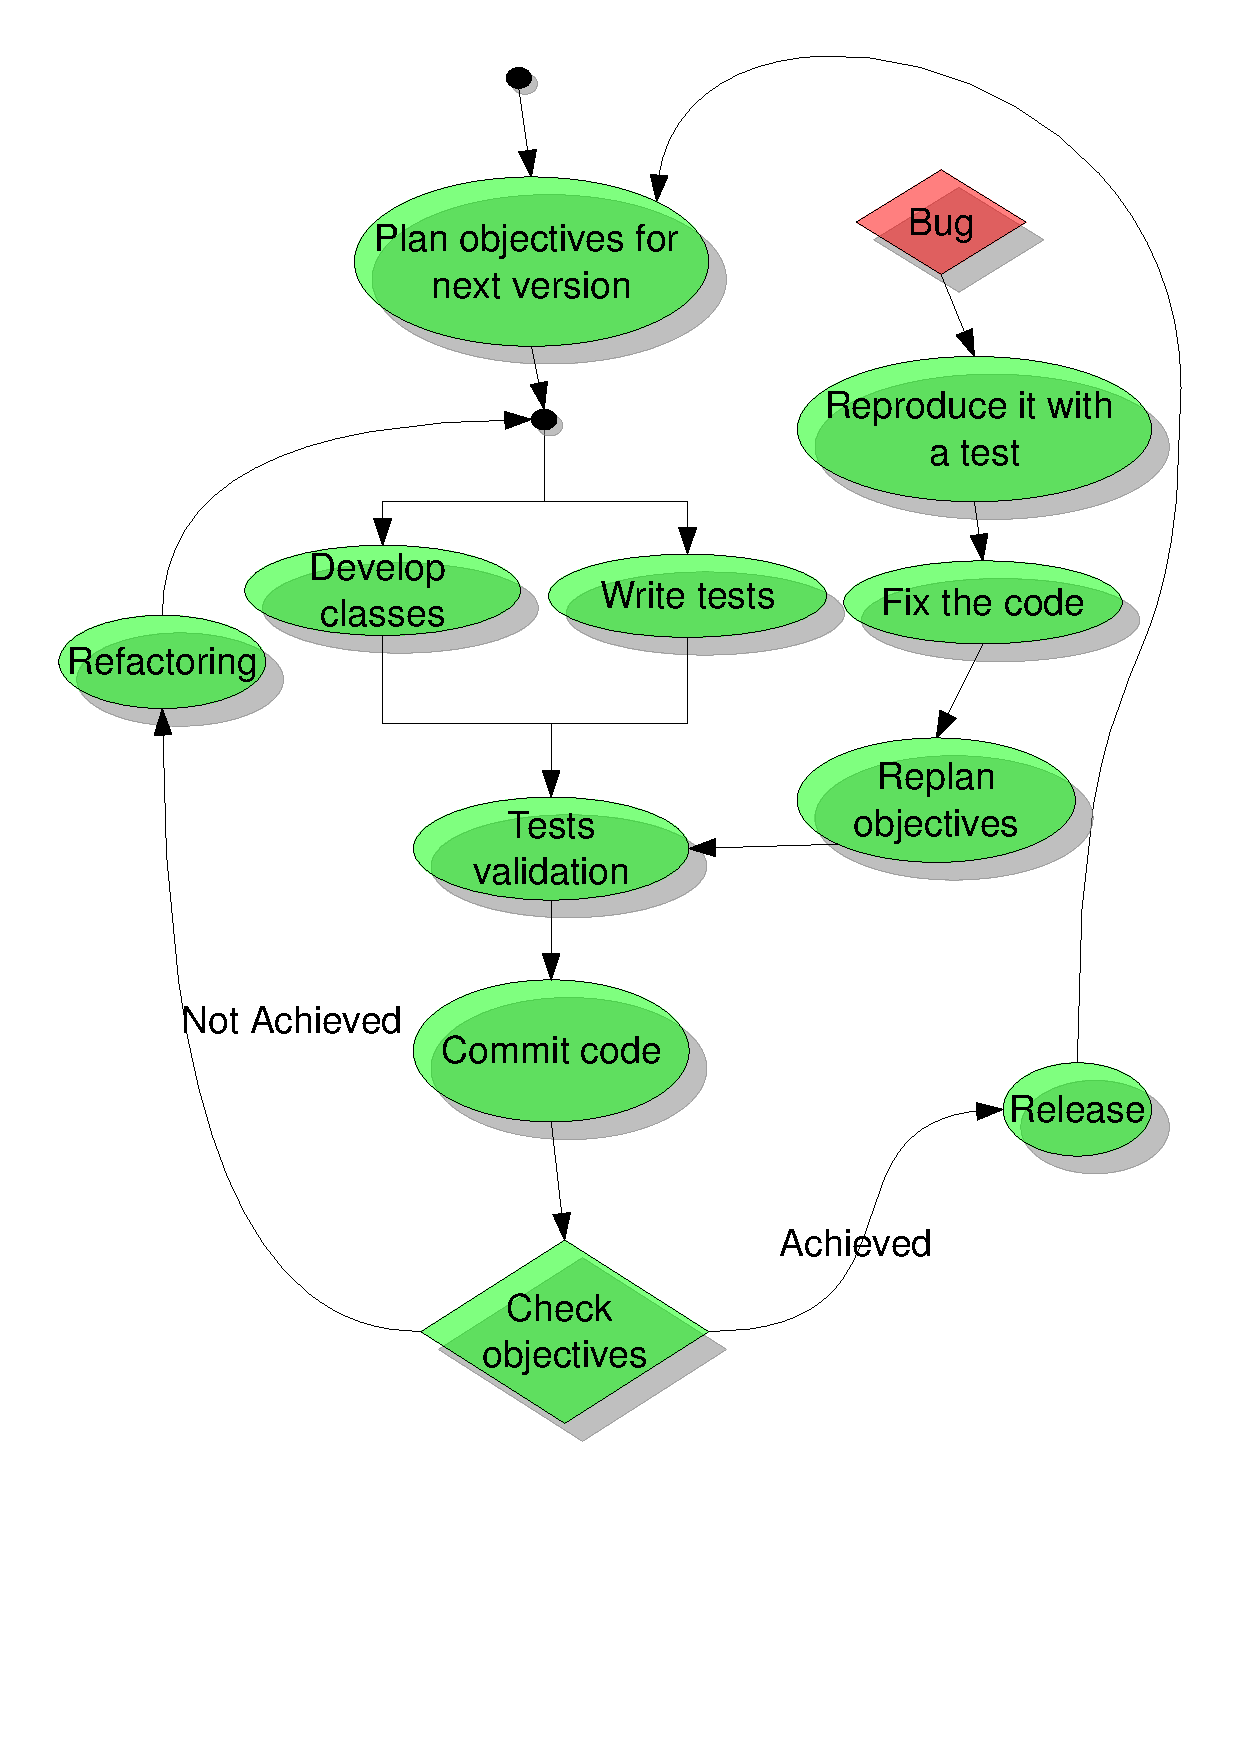
\includegraphics[height=0.9\textheight]{dev_scheme}
  \end{center}
  \caption{Development process}
  \label{figure:dev_proc}
\end{figure}
This document is an introduction to how develop MyServer and interact
with other team members.
The figure \ref{figure:dev_proc} shows the MyServer development
process.
At every loop some objectives are planned and a new release will be
out when they will be completed.
Before the final release is completed, some minors releases are done
on specified dates, no matter if planned objectives are already
completed or not.

This development model is not test-driven because write tests and
develop code are parallel processes.
If somebody finds test-driven a better choice then he or she is free
to adopt it, it is a personal choice, in any case code is committed
to the central repository after it is compilable and it is validated
by all tests.
The central repository at any time must contain a snapshot of the
current development status and it must be compilable and usable.

Differently the bugs fixing process is test driven, when a bug is
detected it should be reproduced by a test.  After the code is
modified to validate all tests, including the new bug test.
Objectives are replanned after a bug fixing because there can be need
to release immediately.

Before the release code can be changed until it reaches a good
readable status.

The communication with other project members is fundamental and when a
message interests everybody then it should be sent on the dev mailing
list, you can find a list of the mailing lists here:
\url{http://www.myserverproject.net/ml.php}.

\begin{section}{Tasks list}
The file TODO in the MyServer directory root contains a list of tasks
that need to be completed.  Each task there should be as simpler as
possible and be very descriptive, in this way new developers can start
working on MyServer without know all its internal mechanisms and
classes.
\end{section}

\begin{section}{Code styling}
\begin{subsection}{Code format}
This simple code snippet shows how format the code and how indent it.
Don't use the tab character to indent it, instead use 2 blank spaces. 
\begin{lstlisting}{language=C++}
//include/foo.h
class Foo
{
public:
  Foo(){}
  int max(int a, int b)
  {
    if(a > b)
      return a;

   return b;
  }
  int longMethod();
private:
  int bar;
};
....
//src/foo.cpp
int Foo::longMethod()
{
...
  return bar;
}
\end{lstlisting}
\end{subsection}

\begin{subsection}{Writing code suggestions}
These are some simple rules to keep in mind writing code:
\begin{itemize}
\item Short methods, avoid long methods.
\item Comments only when there is really need, code should be clean
  itself, have many comments will make it more difficult to maintain
  because any change in the code must be duplicated in the comment.
\item Add a doxygen compatible comment to every method, this is the
  only kind of comment that should be always present, more information
  about doxygen can be found here:
  \url{http://www.stack.nl/~dimitri/doxygen/}.
\item Try to avoid mock objects during testing, base classes can be
  implemented to don't do anything, if you don't know what a mock
  object is then take a look
  here~\url{http://en.wikipedia.org/wiki/Mock_object}.
\item Possibility to use unit testing as code snippets for APIs, tests
  code should be as much clean and readable as possible.
\item Make the code breathe, add blank lines to separe different
  sections and make it clearer.
\end{itemize}
\end{subsection}
\end{section}
\clearpage

\begin{section}{Subversion repository}
\begin{subsection}{Branches}
If there is need to change many things in the source code, like for
example when we implemented an event driven scheduler, that changed
many things in different sections of the code, then it is a good
choice to create a branch from \textit{trunk}.
After the job is completed and the branched version is working well
and it is validated by tests then it will be merged back to the
\textit{trunk} version.
For branches it is not valid the rule that it should work at any time,
they are experimental versions.
\end{subsection}

\begin{subsection}{Access the repository}
You can find information about how access the source code repository here:
\url{http://www.myserverproject.net/subversion.php}
\end{subsection}
\end{section}

\end{document}
